\chapter{Lecture 6}

%--- 信息 ----
\begin{center}
    讲师:王立威 \qquad
    课程时间:25.Mar.25th \qquad 
    笔记:25.June.7th
\end{center}

\bigskip

接着将之前对于离散型随机变量定义的各种熵迁移到连续型随机变量上来 
\begin{definition}[联合微分熵]
    对于两个连续型随机变量$X,Y$,设其联合p.d.f.为$f_{X,Y}(x,y)$,定义其\textbf{联合微分熵}(joint differential entropy)为 
    \[
    h(X, Y) := - \int\int f_{X,Y}(x, y) \log f_{X,Y}(x, y) \dx\dx[y]
    \]
\end{definition}
\begin{definition}[条件微分熵]
    对于两个连续型随机变量$X,Y$,设其联合p.d.f.为$f_{X,Y}(x,y)$,定义其\textbf{条件微分熵}(conditional differential entropy)为 
    \[
    h(X| Y) := - \int\int f_{X,Y}(x, y) \log f_{X|Y}(x, y) \dx\dx[y]
    \]
\end{definition}

下面来讨论一个很重要的量:互信息。 
\begin{definition}[连续型随机变量的互信息]
    对于两个连续型随机变量$X, Y$,具有概率密度$f_{X,Y}, f_{X|Y}, f_{Y|X}$等,定义它们的\textbf{互信息}(mutual information)为 
    \[
    I(X; Y):= h(X) - h(X|Y)
    \]
\end{definition}

这样从形式上定义的互信息竟然保留了离散版本的诸多性质!
\begin{theorem}
    对于两个连续型随机变量$X, Y$,一定有
    \[
    I(X;Y) = h(Y) - h(Y|X) = h(X) + h(Y) - h(X, Y)
    \]

    另外,还可以用联合概率密度和边缘概率密度来表达
    \[
    I(X; Y) = \int\int f_{X,Y}(x, y) \log \dfrac{f_{X,Y}(x,y)}{f_X(x) f_Y(y)} \dx\dx[y]
    \]
\end{theorem}

为什么会造成这样的性质呢?我们考虑它们二者的对应的离散化版本$X_\Delta, Y_\Delta$,会有 
\[
I(X; Y) = \lim_{\Delta\ra 0^+} I(X_\Delta, Y_\Delta)
\]

这说明虽然在连续意义下,微分熵的物理意义不是非常明确,但互信息的物理意义是充分明晰的。

另外,也可以接着定义K-L散度(相对熵)
\begin{definition}
    给定$f,g$分别是连续型随机变量$X,Y$的概率密度函数,定义\textbf{K-L散度}为 
    \[
    \text{KL}(f\| g) := \int f(x) \log \dfrac{f(x)}{g(x)} \dx
    \]
\end{definition}

继续考虑离散化版本$X_\Delta, Y_\Delta$以及他们对应的分布列$P_\Delta, Q_\Delta$。可以发现 
\[
\lim_{\Delta \ra 0^+} \text{KL}(P_\Delta \| Q_\Delta) = \text{KL}(f\| g)
\]

至此,关于信源编码就告一段落了。

现在考虑编码的问题,对于一个随机对象,希望知道最小的描述长度。但这个问题是不平凡的,因为就算是退化到了确定对象也难以严格定义“描述长度”。 好比对于圆,我们可以使用圆心和半径;对于矩形可以使用中心、长和宽;但对于一个比较混沌的图形就难以描述了。

\begin{figure}[H]
    \centering
    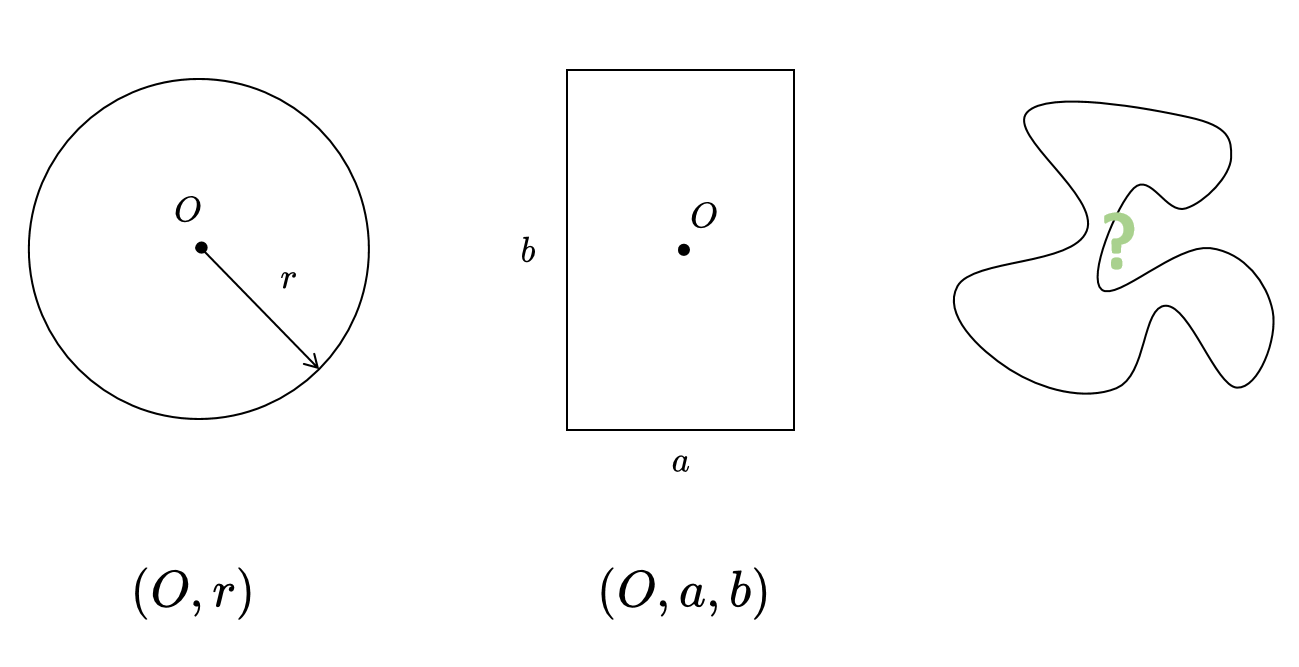
\includegraphics[width=.75\textwidth]{images/c6_1.png}
\end{figure}

这个所谓的“对象”空间太大了,需要限制一下范围,并挖掘本质。 前苏联的数学家Kolmogorov给出了回答,将其限制在了字符串$\{0,1\}^*$当中。

\begin{example}
    直觉上,可以将$000\cdots 0$描述成$n$个0;将$011011011\cdots$描述成$m$个011;但如果原字符串很混乱,那最好的描述不过是将其复述一遍。
\end{example}

这样的直觉需要转为严谨的定义,思考一下就会发现我们需要发掘“计算”的本质。这个问题Turing已经回答了,是“Turing机”(如今的Boole线路与这个模型也是等价的)。那么所有问题都一定有解吗?并不是,证明也很简单。 

\begin{theorem}
    我们考虑所有的决定问题,即给定集合$L \sbe \{0, 1\}^*$,需要对任意的$x\in \{0,1\}^*$判断$x$是否属于$L$。 一定存在某个$L_0$对应的决定问题不存在Turing机上可以解决该问题的算法。
\end{theorem}
\begin{proof}
    记所有的问题构成的集合基数为$\kappa$,记所有算法构成的集合基数为$\lambda$。 对于Turing机,算法本质上就是一个字符串,所以$\lambda$是$\{0, 1\}^*$的基数。而上面的讨论说明了一个$L$可以决定一个问题,故$\kappa$是$\mathcal{P}(\{0, 1\}^*)$的基数。 

    根据Cantor定理,有 
    \[
    \lambda = \card {\{0, 1\}}^* < \card \mathcal{P} \Big( {\{0, 1\}}^* \Big) = \kappa
    \]

    基数不同,所以不存在双射。 因此一定存在一个不可解的问题。
\end{proof}

我们可以讲出这样的不可计算问题,例如说“停机问题”。可以证明:给定算法$A$和输入$i$,不存在算法保证一定可以计算$A$是否可以在有限步内停下。 

Turing的工作其实在一定程度上收到了Godel的启发,在Turing关于计算本质问题的研究工作发表前,Godel证明了任意一阶逻辑的不完备性,也正是熟知的“Godel不完备定理”.